\documentclass[aspectratio=169]{beamer}

\usetheme{metropolis}
\usepackage{graphicx}
\usepackage{booktabs}
\usepackage{amsmath}
\usepackage{amssymb}
\usepackage{tikz}
\usepackage{array}
\usepackage{xcolor}
\usetikzlibrary{positioning, arrows.meta, fit, backgrounds, shapes.geometric}

\graphicspath{{figs/}{../results/figures/}}

% --- Consistent agent colour palette (used across every bar chart and callout) ---
\definecolor{ppoBlue}{HTML}{1f77b4}
\definecolor{srOrange}{HTML}{ff7f0e}
\definecolor{replayGreen}{HTML}{2ca02c}

% Fallback if metropolis theme is not installed -- uncomment the two lines below
% and comment out \usetheme{metropolis}.
% \usetheme{default}
% \usecolortheme{dove}

\title{Vision-Based RL as a Probe of\\Reward, Transition, and Observation Change}
\subtitle{Three architectures, three kinds of change --- PSY~392~CPAI final project}
\author{Shrikrishna Rajule}
\institute{Purdue University}
\date{Spring 2026}

\begin{document}

% ============================================================
% Slide 1 -- Title
% ============================================================
\begin{frame}
  \titlepage
\end{frame}

% ============================================================
% Slide 2 -- The question
% ============================================================
\begin{frame}{The question: three ways the world can change}
  \begin{columns}[T, onlytextwidth]
    \column{0.32\textwidth}
      \centering
      \textbf{Reward moves}\\[0.4em]
      {\Large $\star \rightarrow \star$}\\[0.3em]
      {\small Goal location shifts.\\Dynamics unchanged.}
    \column{0.32\textwidth}
      \centering
      \textbf{Wall appears}\\[0.4em]
      {\Large $\square\mspace{-14mu}{\rule{0.08em}{1.2em}}$}\\[0.3em]
      {\small Transition graph changes.\\Reward unchanged.}
    \column{0.32\textwidth}
      \centering
      \textbf{Observation shifts}\\[0.4em]
      {\Large \textcolor{gray!60}{\textbullet}\,\textcolor{gray!60}{\textbullet}\,\textcolor{gray!60}{\textbullet}}\\[0.3em]
      {\small Pixels differ, state same.\\(Hippocampal remapping.)}
  \end{columns}
  \vspace{0.5em}
  \begin{center}
    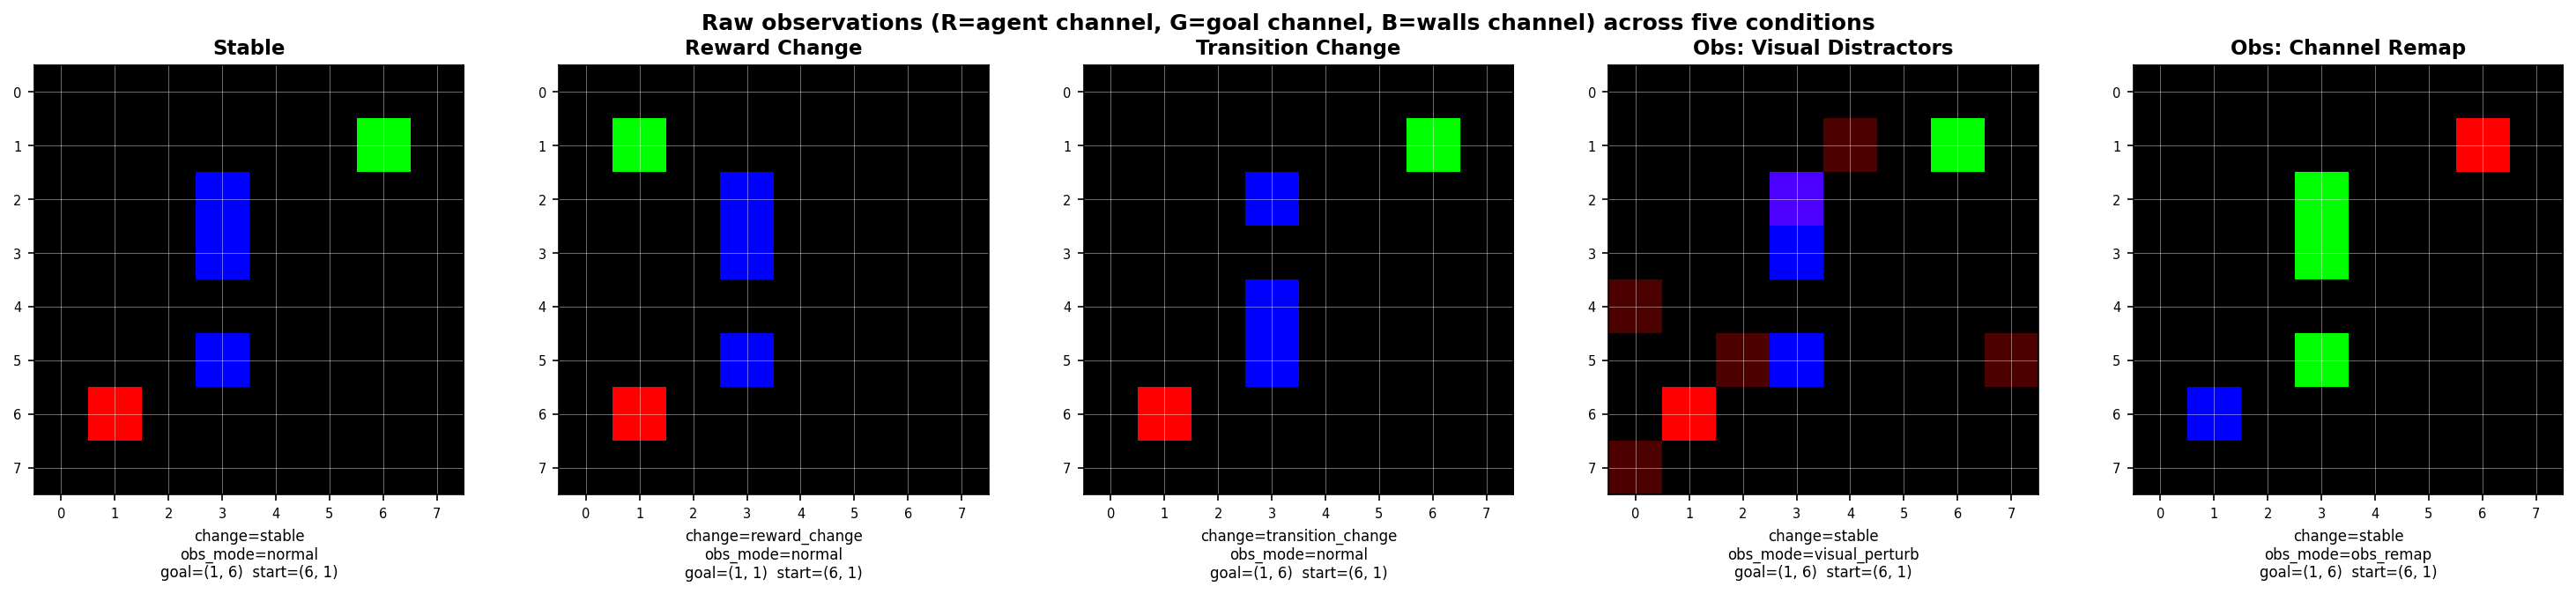
\includegraphics[width=0.82\linewidth]{env_conditions.png}
  \end{center}
  \vspace{-0.3em}
  \centerline{\footnotesize Five conditions, three axes of change. Can three RL architectures tell them apart?}
\end{frame}

% ============================================================
% Slide 3 -- Neuroscience anchor (two cards)
% ============================================================
\begin{frame}{What the neuroscience says}
  \begin{columns}[T]
    \column{0.49\textwidth}
      \begin{block}{Momennejad et al., 2017 \hfill \emph{Nat.\ Hum.\ Behav.}}
        \footnotesize
        Humans revalue \emph{fast} after reward change, \emph{slow} after transition change.\\[0.3em]
        Explained by the Successor Representation:
        \[ Q(s,a) = \langle \psi(s,a),\; \mathbf{w}\rangle \]
        Reward revaluation is just updating $\mathbf{w}$.
      \end{block}
    \column{0.49\textwidth}
      \begin{block}{Sanders, Wilson \& Gershman, 2020 \hfill \emph{eLife}}
        \footnotesize
        Hippocampal remapping as \emph{hidden-state inference}.\\[0.3em]
        \textbf{Rate remapping:} graded change under the same state.\\[0.2em]
        \textbf{Global remapping:} the obs$\rightarrow$state map itself is replaced.
      \end{block}
  \end{columns}
  \vspace{0.6em}
  \centerline{\footnotesize These two papers give me the predictions my five conditions directly operationalize.}
\end{frame}

% ============================================================
% Slide 4 -- Where this builds on the class (class lineage)
% ============================================================
\begin{frame}{Where this builds on the class}
  \centering
  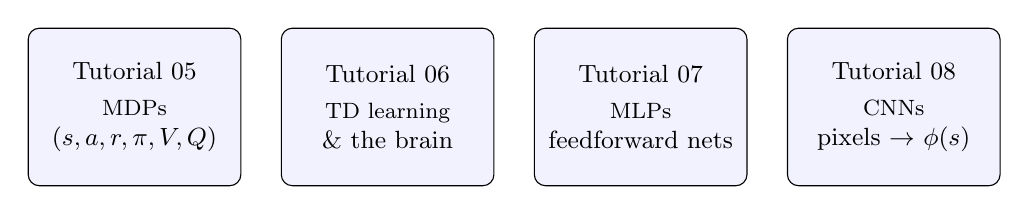
\begin{tikzpicture}[
      tut/.style={draw, rounded corners, minimum width=2.7cm, minimum height=2.0cm, align=center, font=\small, fill=blue!5},
      lbl/.style={font=\footnotesize\bfseries},
      >=Latex,
    ]
    \node[tut] (t5) {\lbl Tutorial 05\\[0.2em]\footnotesize MDPs\\$(s,a,r,\pi,V,Q)$};
    \node[tut, right=0.5cm of t5] (t6) {\lbl Tutorial 06\\[0.2em]\footnotesize TD learning\\\& the brain};
    \node[tut, right=0.5cm of t6] (t7) {\lbl Tutorial 07\\[0.2em]\footnotesize MLPs\\feedforward nets};
    \node[tut, right=0.5cm of t7] (t8) {\lbl Tutorial 08\\[0.2em]\footnotesize CNNs\\pixels $\to$ $\phi(s)$};
  \end{tikzpicture}
  \vspace{1.0em}
  \begin{itemize}\setlength\itemsep{0.1em}\small
    \item Tutorial 05 gave me the MDP vocabulary for describing the task.
    \item Tutorial 06 tied value learning to neuroscience -- the bridge to Momennejad \& Sanders.
    \item Tutorial 07 + 08 gave me the function approximators: MLP heads on top of a CNN encoder.
  \end{itemize}
  \vspace{0.4em}
  \centerline{\footnotesize \textbf{My project adds three different heads on the same encoder and compares what each one learns.}}
\end{frame}

% ============================================================
% Slide 5 -- Three agents, one encoder (annotated with paper citations)
% ============================================================
\begin{frame}{Three agents, one shared CNN encoder}
  \centering
  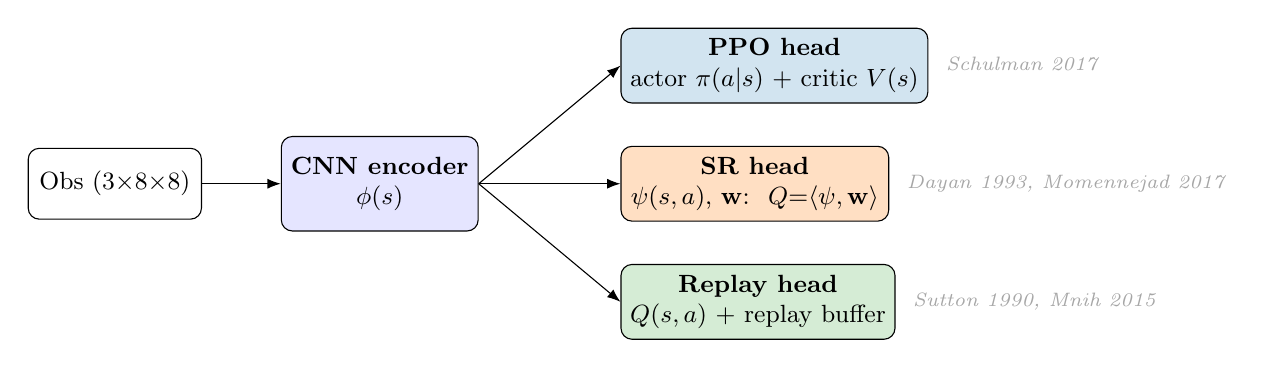
\begin{tikzpicture}[
      node distance=0.8cm and 1.0cm,
      box/.style={draw, rounded corners, minimum width=2.2cm, minimum height=0.9cm, align=center, font=\small},
      encoder/.style={draw, rounded corners, fill=blue!10, minimum width=2.5cm, minimum height=1.2cm, align=center, font=\small\bfseries},
      head/.style={draw, rounded corners, minimum width=3.4cm, minimum height=0.95cm, align=center, font=\small},
      cite/.style={font=\scriptsize\itshape, text=gray!70},
      >=Latex,
    ]
    \node[box] (obs) {Obs (3$\times$8$\times$8)};
    \node[encoder, right=of obs] (enc) {CNN encoder\\$\phi(s)$};
    \node[head, fill=ppoBlue!20, right=1.8cm of enc, yshift=1.5cm] (ppo) {\textbf{PPO head}\\actor $\pi(a|s)$ + critic $V(s)$};
    \node[head, fill=srOrange!25, right=1.8cm of enc] (sr) {\textbf{SR head}\\$\psi(s,a)$, $\mathbf{w}$:\; $Q{=}\langle\psi,\mathbf{w}\rangle$};
    \node[head, fill=replayGreen!20, right=1.8cm of enc, yshift=-1.5cm] (rep) {\textbf{Replay head}\\$Q(s,a)$ + replay buffer};
    \node[cite, right=0.1cm of ppo] {Schulman 2017};
    \node[cite, right=0.1cm of sr]  {Dayan 1993, Momennejad 2017};
    \node[cite, right=0.1cm of rep] {Sutton 1990, Mnih 2015};
    \draw[->] (obs) -- (enc);
    \draw[->] (enc.east) -- (ppo.west);
    \draw[->] (enc.east) -- (sr.west);
    \draw[->] (enc.east) -- (rep.west);
  \end{tikzpicture}
  \vspace{0.3em}
  \centerline{\footnotesize Same pixel$\rightarrow$feature pipeline. Three different credit-assignment mechanisms.}
\end{frame}

% ============================================================
% Slide 6 -- SR in one equation
% ============================================================
\begin{frame}{Successor Representation in one equation}
  \vspace{0.4em}
  \centerline{\Large $Q(s,a) \;=\; \langle\, \psi(s,a),\; \mathbf{w}\,\rangle$}
  \vspace{1.0em}
  \begin{columns}[T, onlytextwidth]
    \column{0.49\textwidth}
      \centering
      \textcolor{srOrange}{\textbf{$\psi(s,a)$}}\\[0.2em]
      ``\emph{where you'll go}''\\[0.1em]
      \small expected discounted future features.\\ Reward-agnostic.
    \column{0.49\textwidth}
      \centering
      \textcolor{srOrange}{\textbf{$\mathbf{w}$}}\\[0.2em]
      ``\emph{what you want}''\\[0.1em]
      \small the reward weights.\\ Updated \emph{independently} of $\psi$.
  \end{columns}
  \vspace{1.0em}
  \begin{alertblock}{The one-line trick}
    \centerline{\textbf{When reward changes: update $\mathbf{w}$, keep $\psi$.}}
    \small\centerline{This is Momennejad 2017's prediction. My \texttt{wonly} variant tests it directly.}
  \end{alertblock}
\end{frame}

% ============================================================
% Slide 7 -- Five conditions (with axis legend)
% ============================================================
\begin{frame}{Environment: one grid, five conditions}
  \centering
  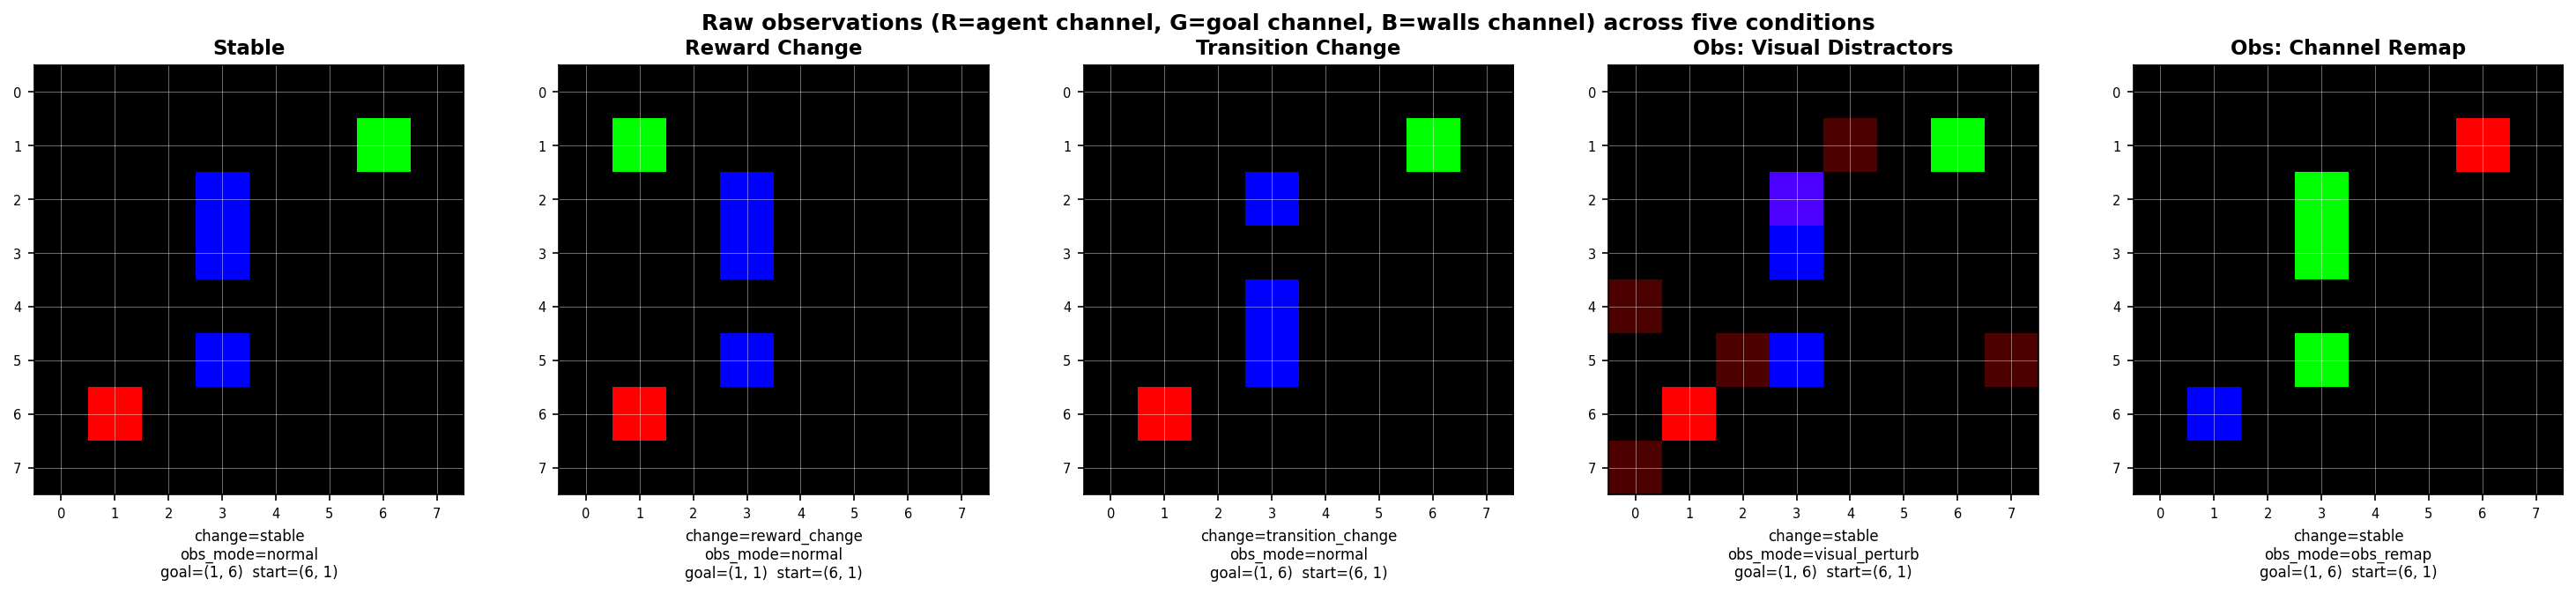
\includegraphics[width=0.92\linewidth]{env_conditions.png}\\[0.6em]
  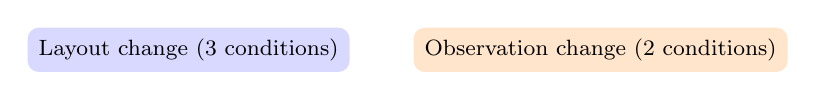
\begin{tikzpicture}[font=\footnotesize]
    \node[fill=blue!15, rounded corners, inner sep=4pt] (A) {Layout change (3 conditions)};
    \node[fill=orange!20, rounded corners, inner sep=4pt, right=0.8cm of A] (B) {Observation change (2 conditions)};
  \end{tikzpicture}
  \vspace{0.3em}
  \centerline{\footnotesize \texttt{stable}, \texttt{reward\_change}, \texttt{transition\_change} $|$ \texttt{obs\_visual} (rate), \texttt{obs\_remap} (global)}
\end{frame}

% ============================================================
% Slide 8 -- Five hypotheses (card grid)
% ============================================================
\begin{frame}{Five hypotheses -- who should win where?}
  \centering
  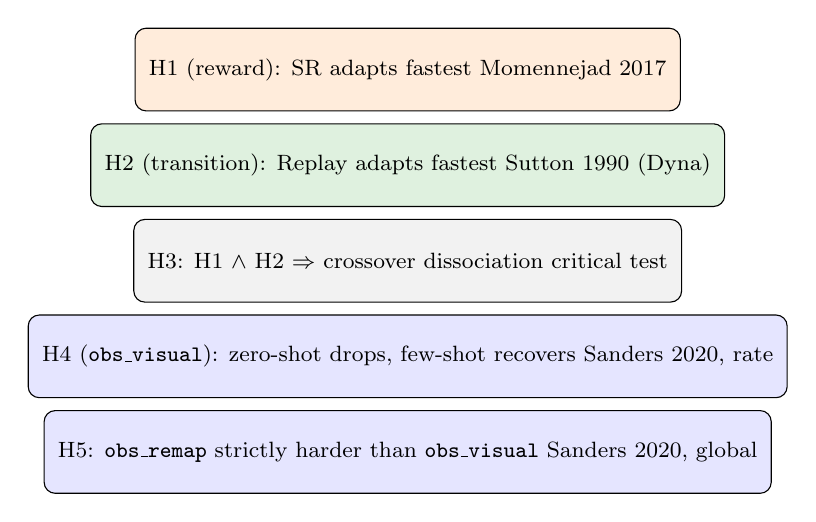
\begin{tikzpicture}[
      card/.style={draw, rounded corners, minimum width=5.6cm, minimum height=1.05cm, align=left, font=\footnotesize, inner sep=5pt},
      winner/.style={font=\footnotesize\bfseries},
      basis/.style={font=\scriptsize\itshape, text=gray!65},
    ]
    \node[card, fill=srOrange!15] (h1) {\winner H1 (reward): SR adapts fastest \hfill \basis Momennejad 2017};
    \node[card, fill=replayGreen!15, below=0.15cm of h1] (h2) {\winner H2 (transition): Replay adapts fastest \hfill \basis Sutton 1990 (Dyna)};
    \node[card, fill=gray!10, below=0.15cm of h2] (h3) {\winner H3: H1 $\wedge$ H2 $\Rightarrow$ crossover dissociation \hfill \basis critical test};
    \node[card, fill=blue!10, below=0.15cm of h3] (h4) {\winner H4 (\texttt{obs\_visual}): zero-shot drops, few-shot recovers \hfill \basis Sanders 2020, rate};
    \node[card, fill=blue!10, below=0.15cm of h4] (h5) {\winner H5: \texttt{obs\_remap} strictly harder than \texttt{obs\_visual} \hfill \basis Sanders 2020, global};
  \end{tikzpicture}
  \vspace{0.4em}
  \centerline{\footnotesize Each results slide maps back to one of these five.}
\end{frame}

% ============================================================
% Slide 9 -- Protocol & metrics
% ============================================================
\begin{frame}{Protocol and metrics}
  \begin{columns}[T, onlytextwidth]
    \column{0.55\textwidth}
      \textbf{Two phases per (agent, seed):}
      \begin{enumerate}\setlength\itemsep{0.1em}\small
        \item Train on \texttt{stable} to convergence.
        \item \textbf{Zero-shot eval} on all 5 conditions.
        \item \textbf{Few-shot adaptation} on each changed condition (20 PPO batches / 60 SR, Replay episodes).
      \end{enumerate}
      \small 3 seeds $\times$ 3 agents $\times$ 5 conditions.
    \column{0.45\textwidth}
      \textbf{Four metrics:}
      \begin{itemize}\setlength\itemsep{0.1em}\small
        \item Greedy-success rate (snapshot).
        \item \textbf{AUC} of success over adaptation window.
        \item \textbf{$t_{0.5}$}: first step with success $\geq 0.5$.
        \item \textbf{Linear probe} on CNN features (agent pos, goal id, distance).
      \end{itemize}
  \end{columns}
\end{frame}

% ============================================================
% Slide 10 -- Stable training converges (NEW)
% ============================================================
\begin{frame}{Stable training: all three agents converge}
  \centering
  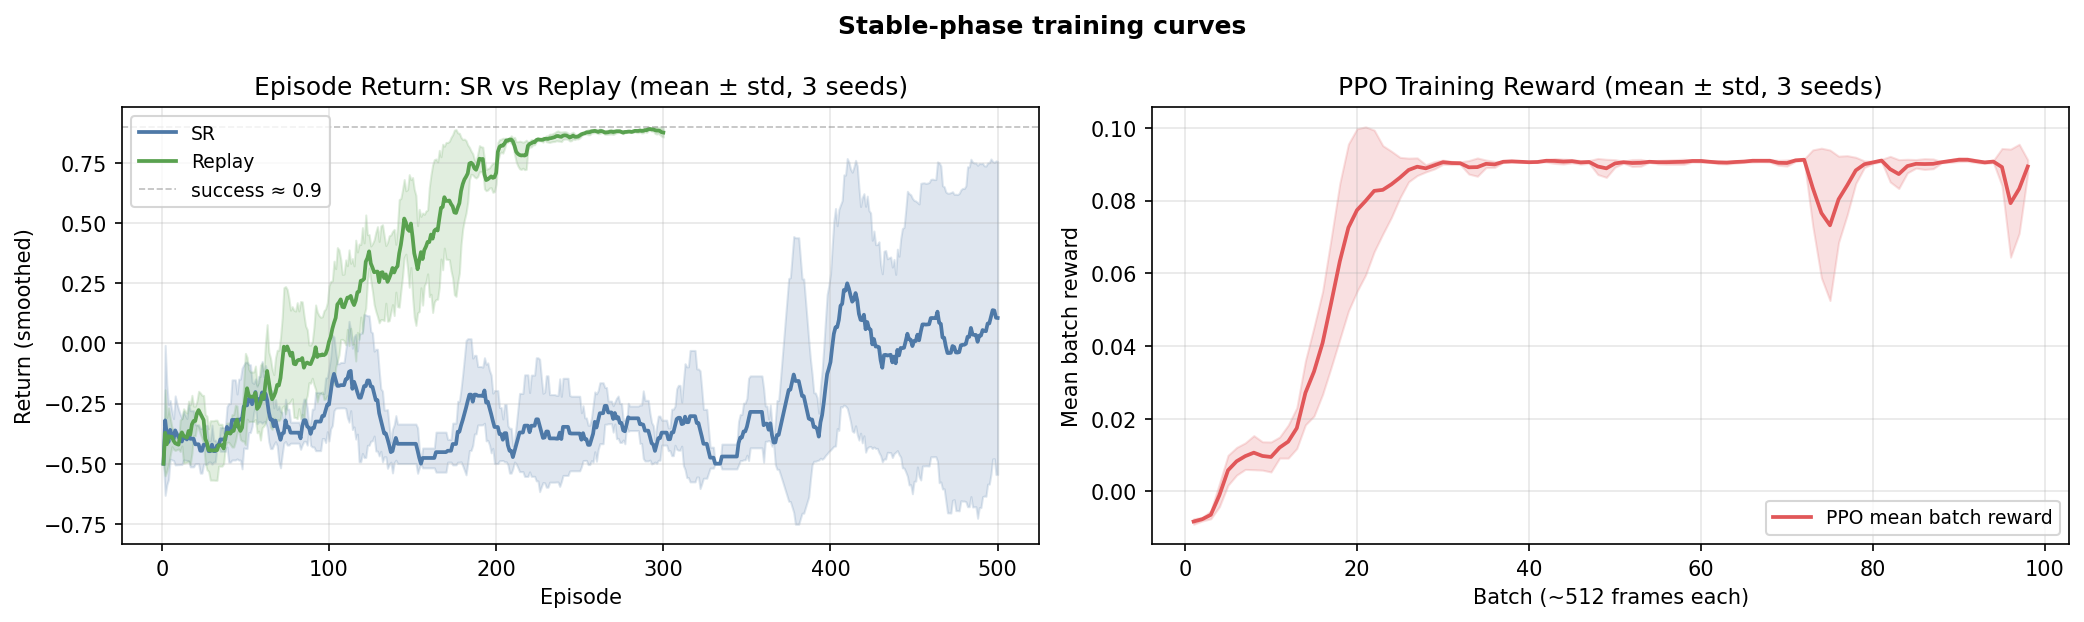
\includegraphics[width=0.82\linewidth]{training_curves.png}\\[0.3em]
  \footnotesize
  PPO converges in $\sim$10 batches; Replay by $\sim$150 episodes; SR hits transient 1.0 peaks
  mid-training but regresses.
  \vspace{0.3em}
  \centerline{\textbf{This is the floor the adaptation phase starts from.}}
\end{frame}

% ============================================================
% Slide 11 -- Zero-shot: who generalizes? (NEW)
% ============================================================
\begin{frame}{Zero-shot: who generalizes?}
  \centering
  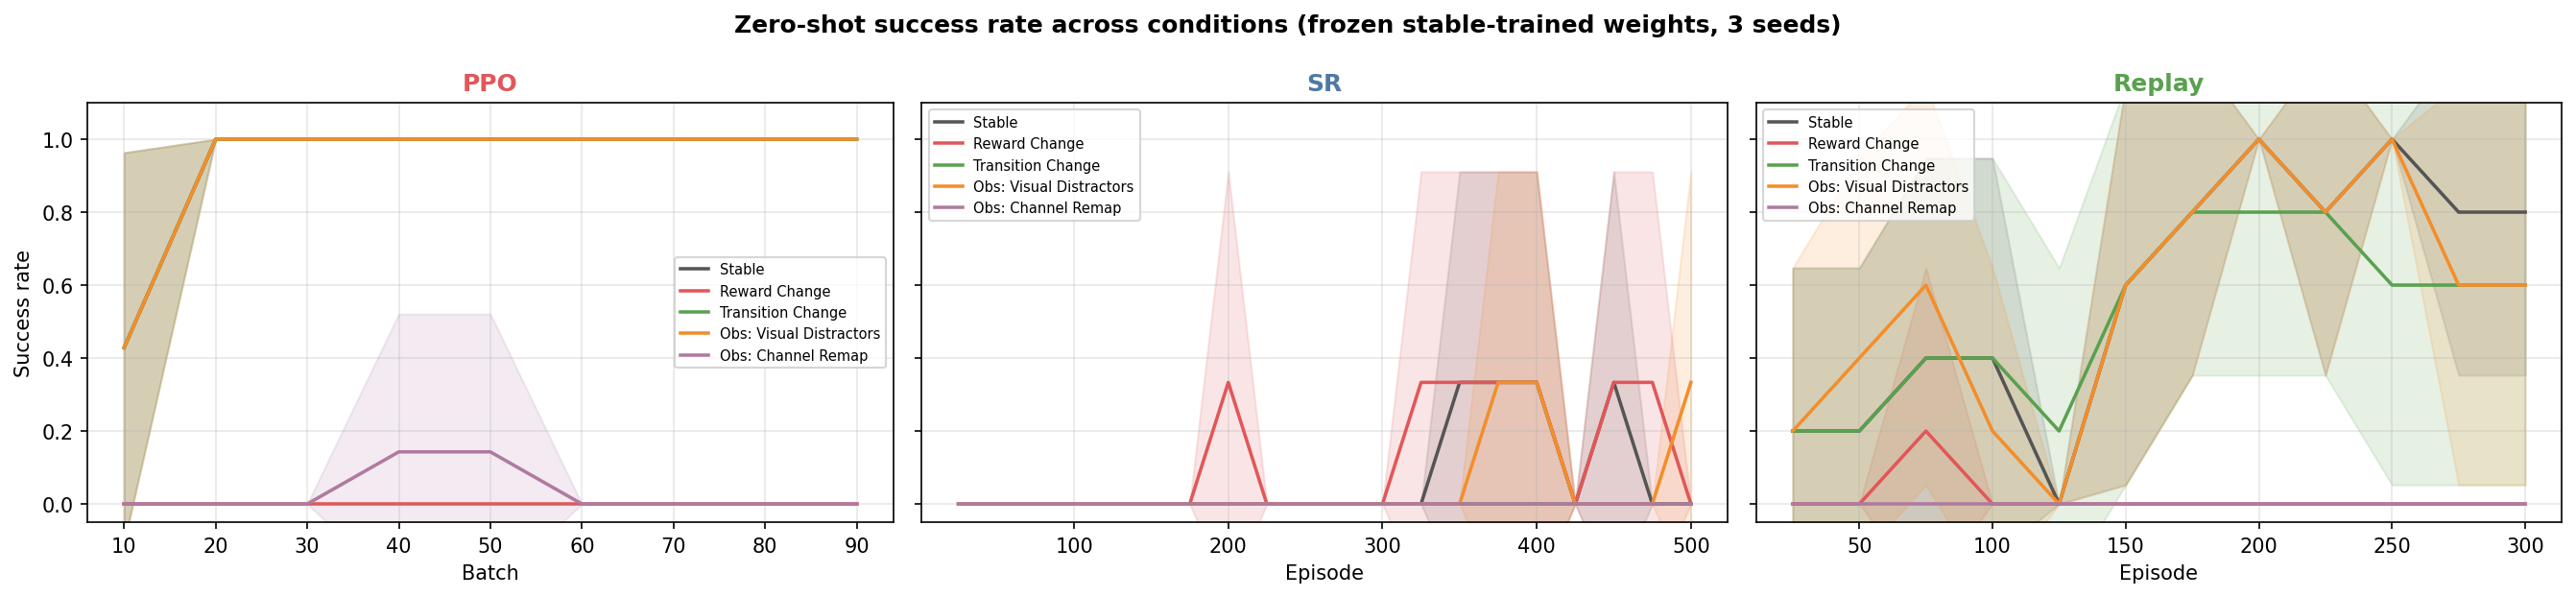
\includegraphics[width=0.9\linewidth]{zero_shot_eval.png}\\[0.3em]
  \footnotesize
  \begin{itemize}\setlength\itemsep{0.05em}
    \item PPO ceiling on \texttt{stable}, \texttt{transition}, \texttt{obs\_visual}; floor on \texttt{reward\_change}, \texttt{obs\_remap}.
    \item Replay: ceiling on \texttt{stable}; $2/3$ seeds generalize on \texttt{transition} and \texttt{obs\_visual}; floor on \texttt{reward\_change}, \texttt{obs\_remap}.
    \item SR at or near floor everywhere -- foreshadows the column-discrimination problem we diagnose on slide 14.
  \end{itemize}
\end{frame}

% ============================================================
% Slide 12 -- Few-shot adaptation (was slide 10)
% ============================================================
\begin{frame}{Few-shot adaptation -- Replay dominates (H2, H4, H5)}
  \centering
  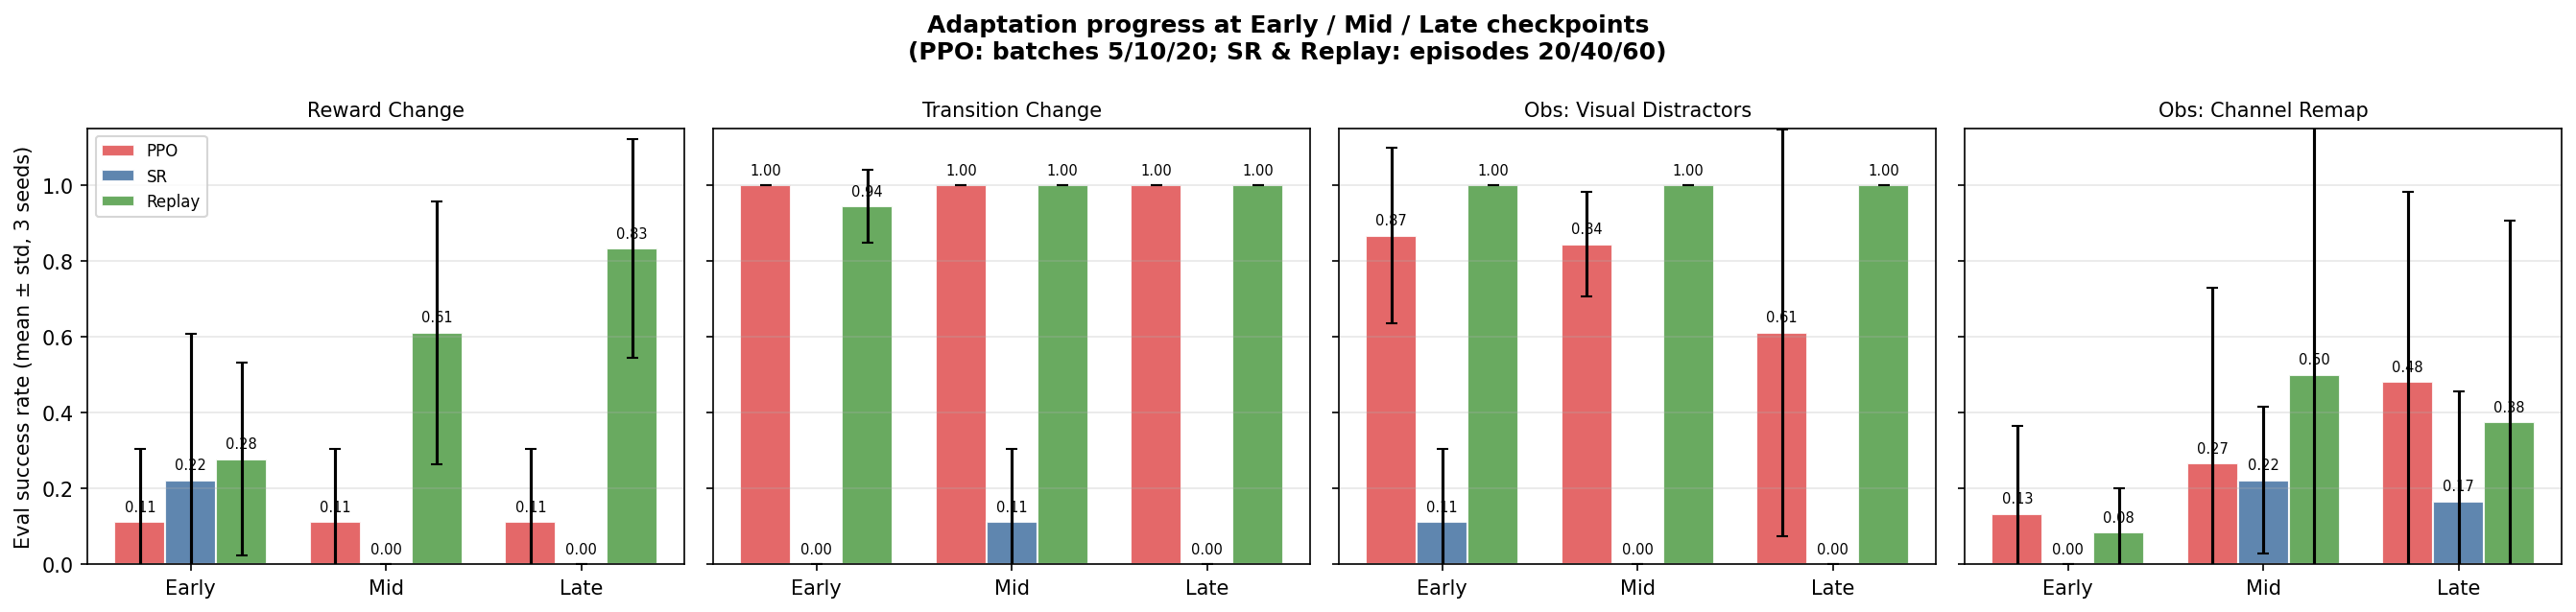
\includegraphics[width=0.78\linewidth]{cross_agent_adaptation.png}\\[0.2em]
  \footnotesize
  \begin{itemize}\setlength\itemsep{0.05em}
    \item \textbf{H2 directionally supported}: Replay and PPO both reach $1.00$ on \texttt{transition\_change} -- a tie near ceiling.
    \item \textbf{H4 supported for Replay} ($0.67 \rightarrow 1.00$ on \texttt{obs\_visual}, rate remapping); partial for PPO ($1.00 \rightarrow 0.56$, stable-LR fine-tune regression).
    \item \textbf{H5 supported for Replay} ($0.50$ vs $1.00$); PPO ties; SR near floor on both.
  \end{itemize}
\end{frame}

% ============================================================
% Slide 13 -- The Momennejad signal (AUC bar chart)
% ============================================================
\begin{frame}{The Momennejad signal hiding in the data}
  \centering
  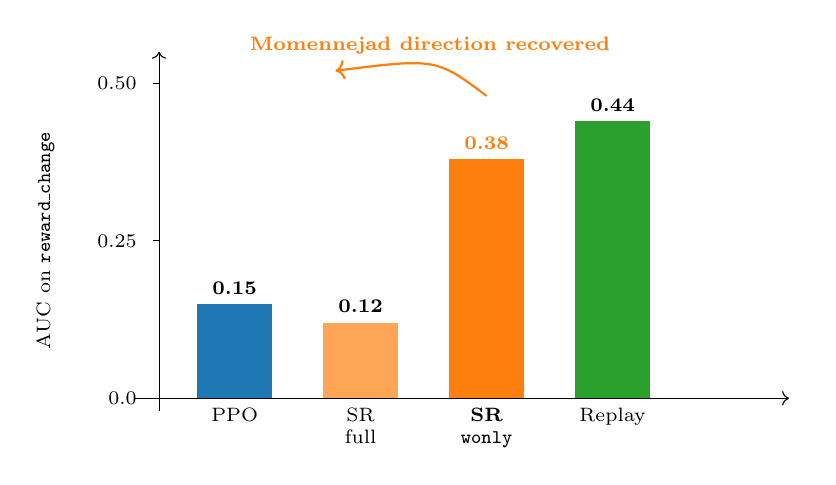
\begin{tikzpicture}[x=1.6cm, y=0.08cm, font=\small]
    % axis
    \draw[->] (-0.2,0) -- (5.0,0) node[right]{};
    \draw[->] (0,-2) -- (0,55) node[above]{};
    % y-axis ticks
    \foreach \y in {0, 25, 50} {
      \draw (-0.05,\y) -- (0,\y);
      \node[left, font=\scriptsize] at (-0.1, \y) {0.\y};
    }
    \node[rotate=90, font=\scriptsize] at (-0.9, 25) {AUC on \texttt{reward\_change}};
    % bars
    \fill[ppoBlue]       (0.30,0) rectangle (0.90,15);
    \fill[srOrange!70]   (1.30,0) rectangle (1.90,12);
    \fill[srOrange]      (2.30,0) rectangle (2.90,38);
    \fill[replayGreen]   (3.30,0) rectangle (3.90,44);
    % value labels on top
    \node[above, font=\scriptsize\bfseries] at (0.60, 15) {0.15};
    \node[above, font=\scriptsize\bfseries] at (1.60, 12) {0.12};
    \node[above, font=\scriptsize\bfseries] at (2.60, 38) {\textcolor{srOrange}{\textbf{0.38}}};
    \node[above, font=\scriptsize\bfseries] at (3.60, 44) {0.44};
    % x-axis labels
    \node[below, font=\scriptsize, align=center] at (0.60, 0) {PPO};
    \node[below, font=\scriptsize, align=center] at (1.60, 0) {SR\\full};
    \node[below, font=\scriptsize\bfseries, align=center] at (2.60, 0) {SR\\\texttt{wonly}};
    \node[below, font=\scriptsize, align=center] at (3.60, 0) {Replay};
    % call-out arrow
    \draw[->, thick, srOrange] (2.60, 48) .. controls (2.2, 54) .. (1.4, 52)
      node[midway, above, font=\scriptsize\bfseries]{\color{srOrange}Momennejad direction recovered};
  \end{tikzpicture}
  \vspace{0.3em}
  \centerline{\footnotesize The end-of-phase snapshot table said ``SR $=0$''. The AUC view says: \textbf{SR-\texttt{wonly} $>$ PPO}, approaches Replay.}
  \centerline{\footnotesize \textbf{H1 partially supported} -- the signal was hidden by transient regression, not absent.}
\end{frame}

% ============================================================
% Slide 14 -- Probe + diagnosis (merged)
% ============================================================
\begin{frame}{The probe tells us what SR actually learned}
  \begin{columns}[T]
    \column{0.42\textwidth}
      \centering
      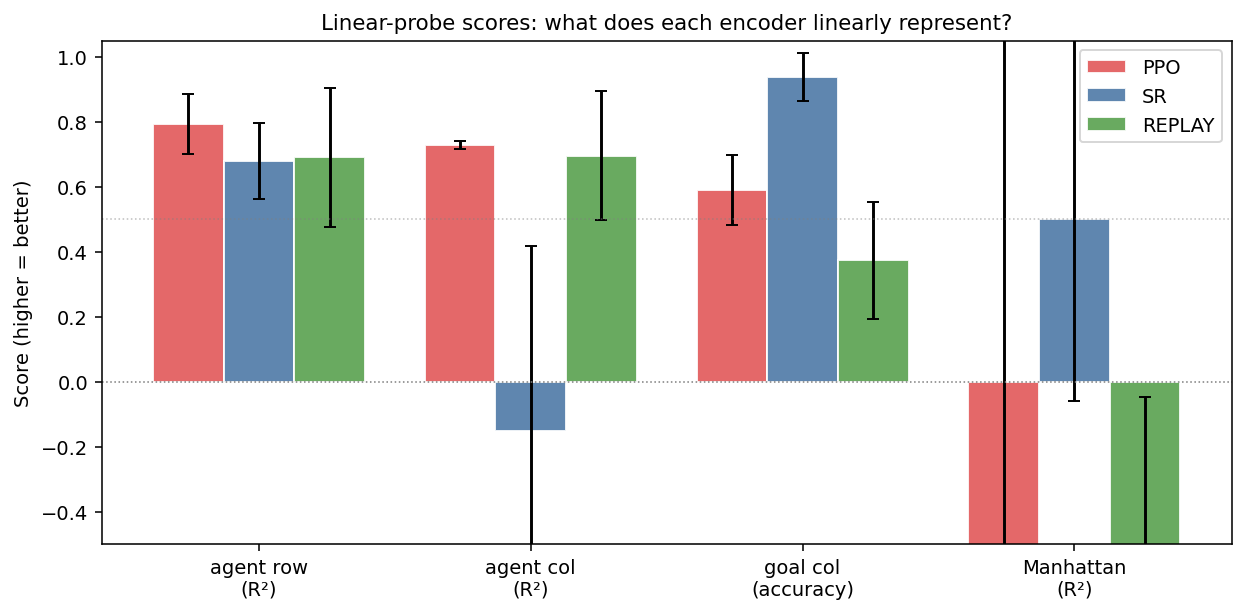
\includegraphics[width=\linewidth]{representation_probe.png}\\[0.2em]
      {\scriptsize mean across seeds; $R^2$ except goal-col = accuracy.}
    \column{0.56\textwidth}
      \footnotesize
      \begin{tabular}{@{}l c c c@{}}
        \toprule
        Target & PPO & \textcolor{srOrange}{\textbf{SR}} & Replay \\
        \midrule
        agent row $R^2$  & $0.79$ & $0.68$ & $0.69$ \\
        agent col $R^2$  & $0.73$ & \textcolor{srOrange}{$\mathbf{-0.15}$} & $0.70$ \\
        goal col acc     & $0.59$ & \textcolor{srOrange}{$\mathbf{0.94}$}   & $0.37$ \\
        Manhattan $R^2$  & $-3.1$ & \textcolor{srOrange}{$\mathbf{+0.50}$}  & $-1.4$ \\
        \bottomrule
      \end{tabular}
      \vspace{0.5em}

      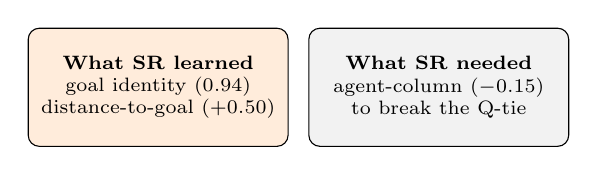
\begin{tikzpicture}[
          cell/.style={draw, rounded corners, minimum width=3.3cm, minimum height=1.5cm, align=center, font=\scriptsize},
        ]
        \node[cell, fill=srOrange!15] (L) {\textbf{What SR learned}\\goal identity ($0.94$)\\distance-to-goal ($+0.50$)};
        \node[cell, fill=gray!10, right=0.25cm of L] (N) {\textbf{What SR needed}\\agent-column ($-0.15$)\\to break the Q-tie};
      \end{tikzpicture}
  \end{columns}
  \vspace{0.2em}
  \centerline{\footnotesize \textbf{Diagnosis: deep-SF policy-extraction fragility, not representation collapse.}\; Fix: action-conditioned $\phi(s,a)$ + Q-margin term (Barreto 2017, Lehnert 2024).}
\end{frame}

% ============================================================
% Slide 15 -- Takeaways
% ============================================================
\begin{frame}{Takeaways \& what's next}
  \begin{itemize}\setlength\itemsep{0.4em}
    \item \textbf{Five-condition testbed} cleanly separates reward / transition / observation change.
    \item \textbf{H2, H4, H5 supported in direction} -- most cleanly for Replay. H1 supported via AUC; H3 not.
    \item \textbf{Probe-as-diagnostic:} turned an ambiguous SR result into an architectural finding.
    \item \textbf{Future work:} action-conditioned $\phi(s,a)$; Q-margin term; adaptation-phase LR tuning for PPO.
  \end{itemize}
  \vspace{0.8em}
  \centerline{\Large\textbf{Thank you --- questions?}}
\end{frame}

% ============================================================
% Backup slides
% ============================================================
\appendix
\begin{frame}{Backup: full adaptation grid}
  \centering
  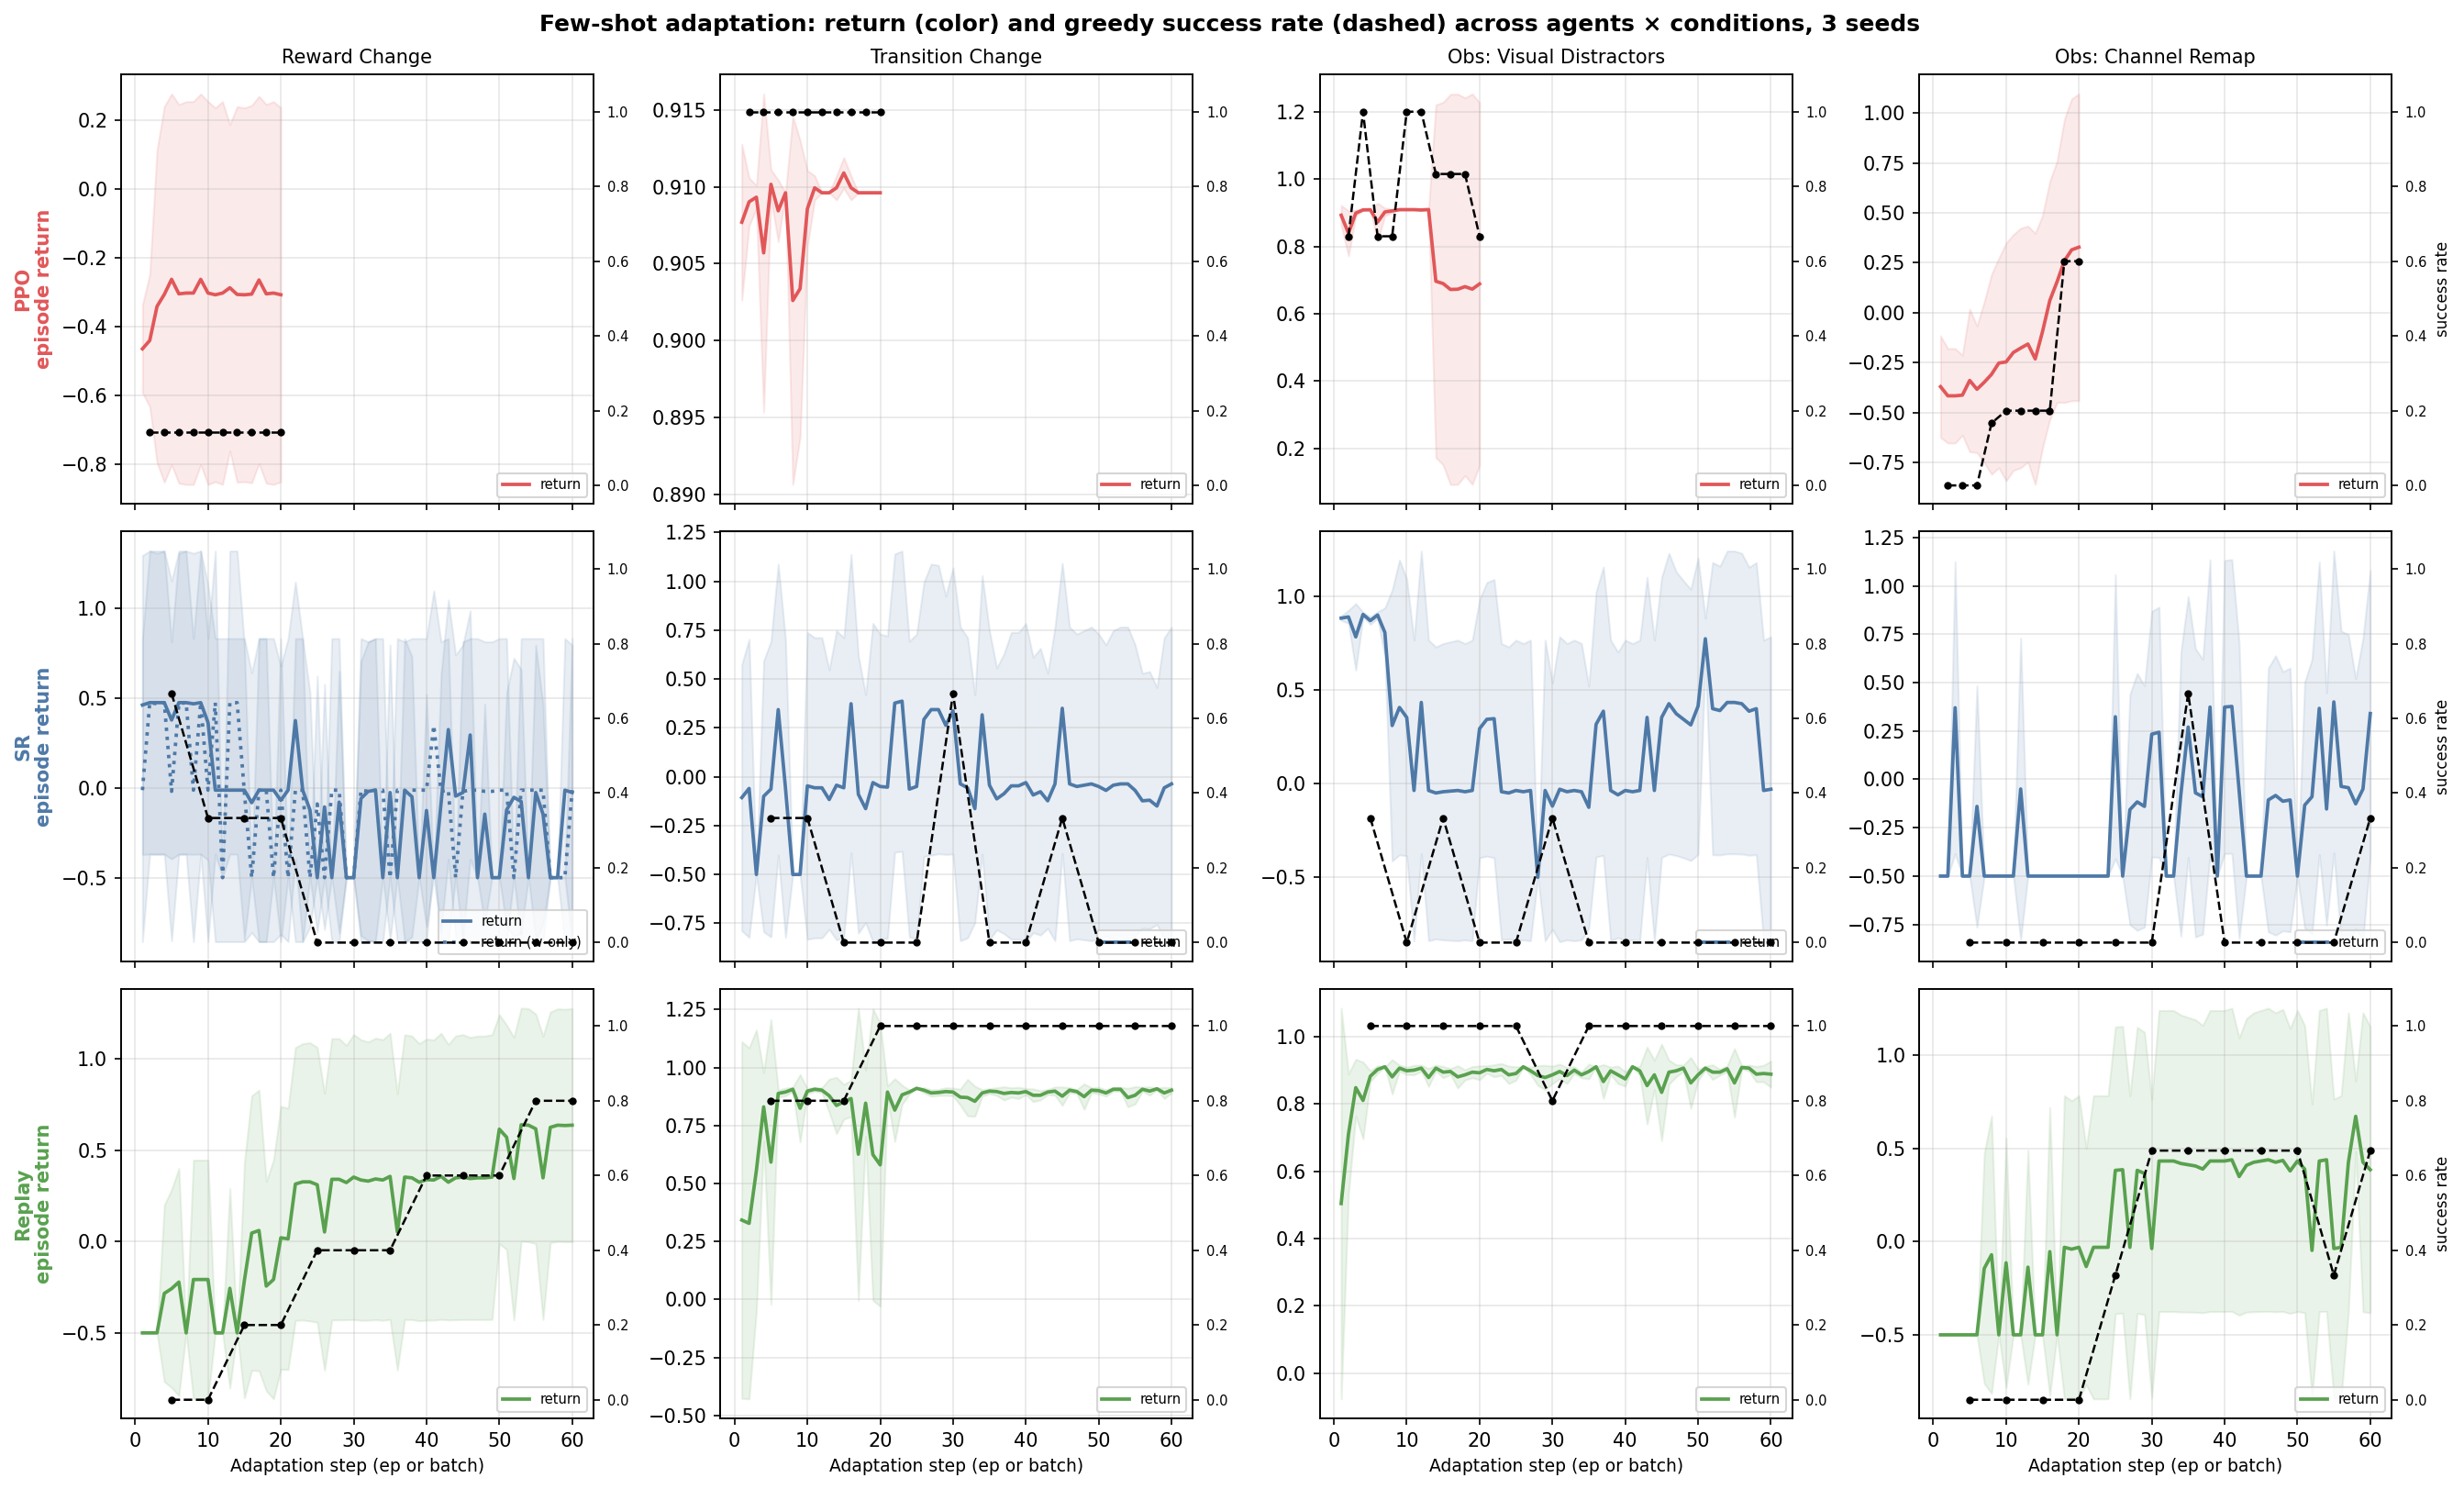
\includegraphics[width=0.82\linewidth]{adaptation_grid.png}
\end{frame}

\begin{frame}{Backup: $\phi$-normalization ablation (Lehnert 2024)}
  \centering
  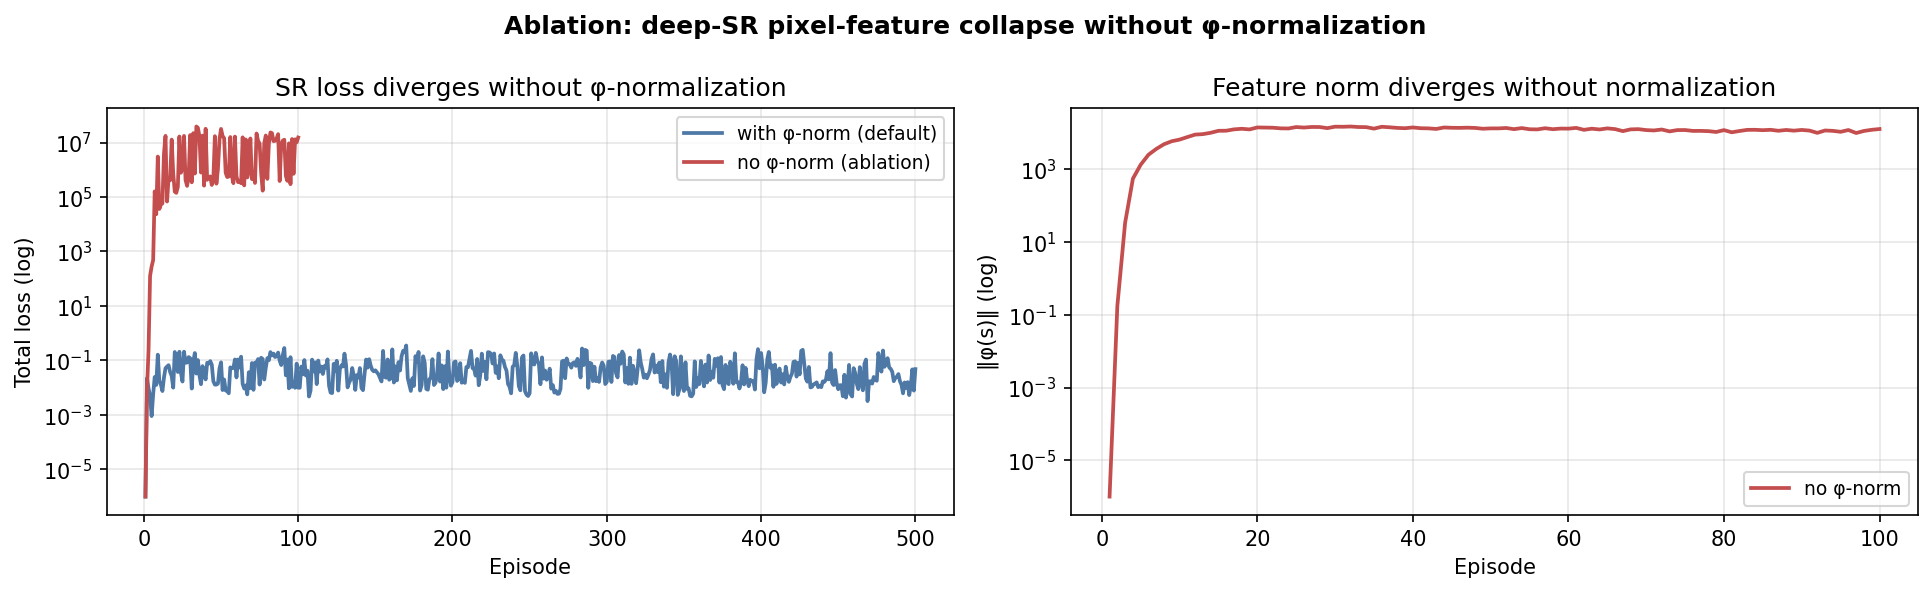
\includegraphics[width=0.72\linewidth]{ablation_sr_no_norm.png}\\[0.3em]
  \small Without normalization, $\|\phi\|$ and SR-Bellman MSE diverge by $\sim 10^7$ within 100 episodes.
\end{frame}

\end{document}
